
\begin{frame}[fragile]{Proposed Method: H-Algorithm}
  \begin{center}
    \vspace{-1cm}
\begin{figure}
  \centering
  \subfloat{ 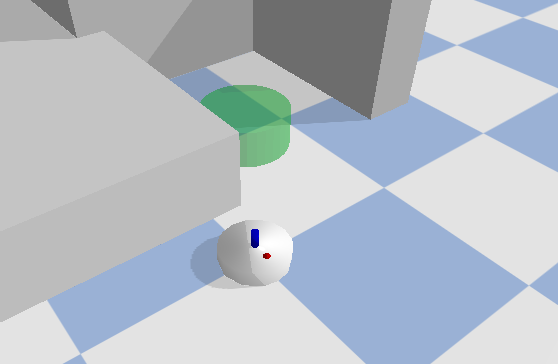
\includegraphics[width=0.45\textwidth]{figures/proposed_method/robot_to_target}}\quad
  \subfloat{ 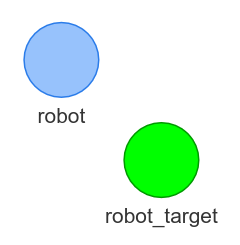
\includegraphics[width=0.35\textwidth]{figures/proposed_method/connecting_nodes/robot_to_target/robot_to_target}}
\end{figure}
  \end{center}
\end{frame}


\begin{frame}[fragile]{Proposed Method: H-Algorithm}
  \begin{center}
    \vspace{-1cm}
\begin{figure}
  \centering
  \subfloat{ 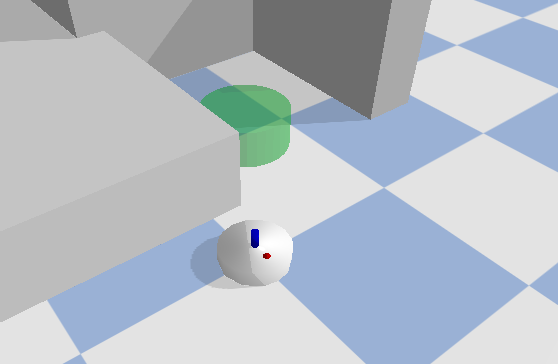
\includegraphics[width=0.45\textwidth]{figures/proposed_method/robot_to_target}}\quad
  \subfloat{ 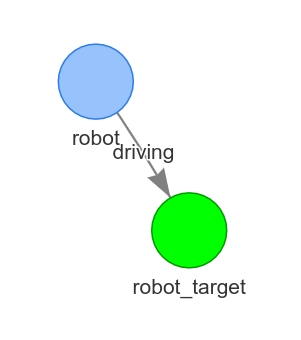
\includegraphics[width=0.35\textwidth]{figures/proposed_method/connecting_nodes/robot_to_target/robot_drive_target}}
\end{figure}
  \end{center}
\end{frame}


\begin{frame}[fragile]{Proposed Method: H-Algorithm}

    \vspace{-1cm}
  \begin{center}
\begin{figure}
  \centering
  \subfloat{ 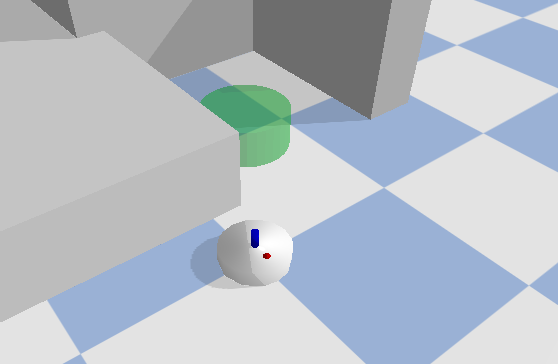
\includegraphics[width=0.45\textwidth]{figures/proposed_method/robot_to_target}}\quad
  \subfloat{ 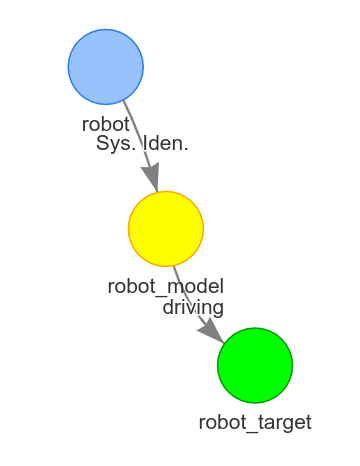
\includegraphics[width=0.35\textwidth]{figures/proposed_method/connecting_nodes/robot_to_target/robot_iden_drive_target}}
\end{figure}
  \end{center}
\end{frame}

\begin{frame}[fragile]{Proposed Method: H-Algorithm}

    \vspace{-1cm}
  \begin{center}
\begin{figure}
  \centering
  \subfloat{ 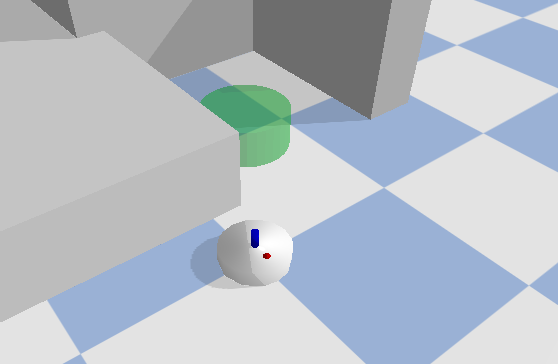
\includegraphics[width=0.45\textwidth]{figures/proposed_method/robot_to_target}}\quad
  \subfloat{ 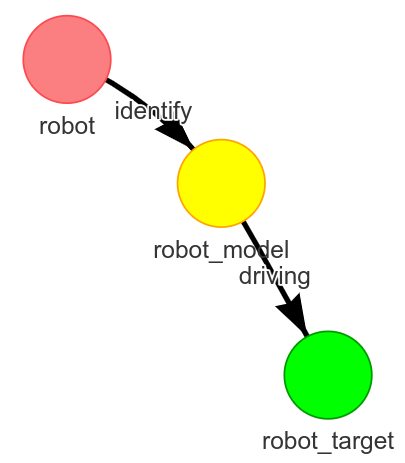
\includegraphics[width=0.35\textwidth]{figures/proposed_method/connecting_nodes/robot_to_target/execute_robot_to_target_1}}
\end{figure}
  \end{center}
\end{frame}

\begin{frame}[fragile]{Proposed Method: H-Algorithm}
    \vspace{-1cm}
  \begin{center}
\begin{figure}
  \centering
  \subfloat{ 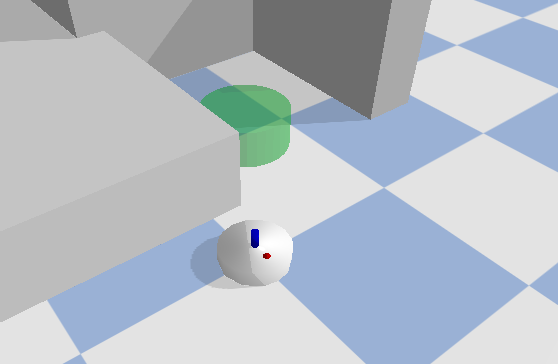
\includegraphics[width=0.45\textwidth]{figures/proposed_method/robot_to_target}}\quad
  \subfloat{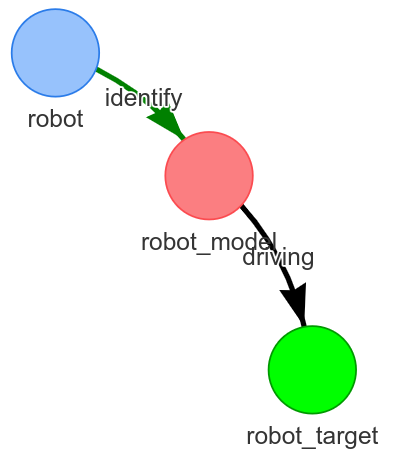
\includegraphics[width=0.35\textwidth]{figures/proposed_method/connecting_nodes/robot_to_target/execute_robot_to_target_2}}
\end{figure}
  \end{center}
\end{frame}

\begin{frame}[fragile]{Proposed Method: H-Algorithm}

    \vspace{-1cm}
  \begin{center}
\begin{figure}
  \centering
  \subfloat{ 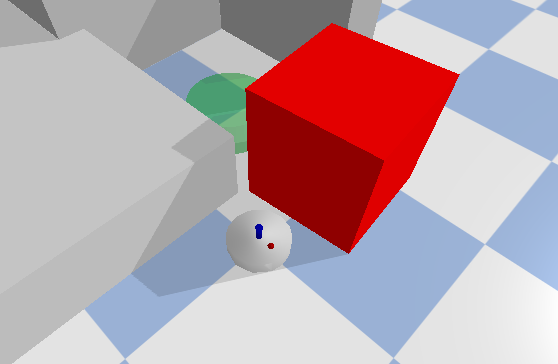
\includegraphics[width=0.45\textwidth]{figures/proposed_method/robot_to_target_obj}}\quad
  \subfloat{ 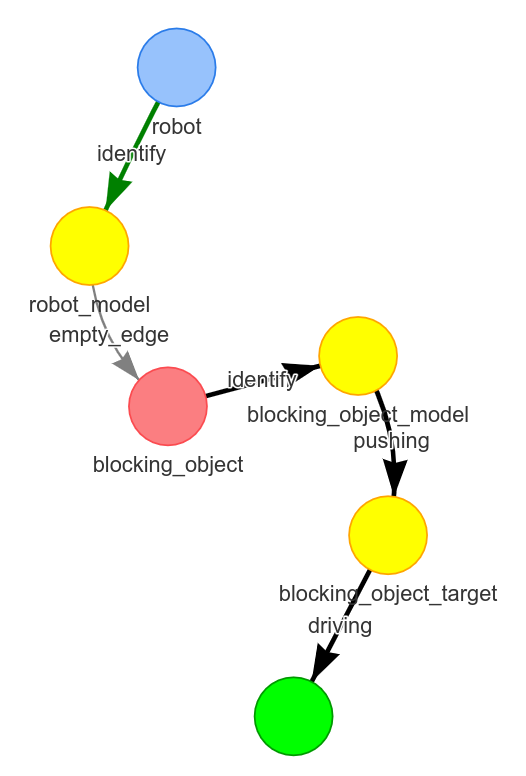
\includegraphics[width=0.3\textwidth]{figures/proposed_method/connecting_nodes/blocking_obj/blocking_obj_3}}
\end{figure}
  \end{center}
\end{frame}

\begin{frame}[fragile]{Proposed Method: H-Algorithm}
    \vspace{-1cm}
  \begin{center}
\begin{figure}
  \centering
  \subfloat{ 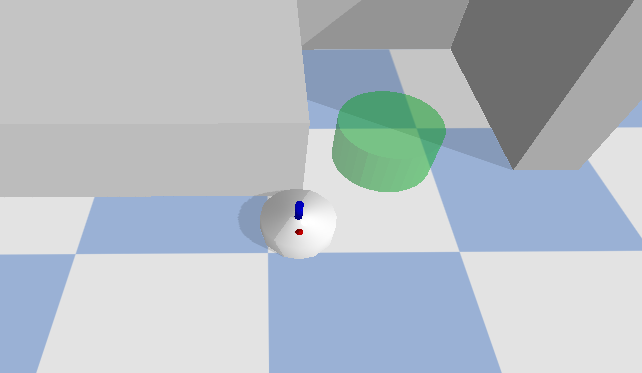
\includegraphics[width=0.45\textwidth]{figures/proposed_method/robot_to_target_execute}}\quad
  \subfloat{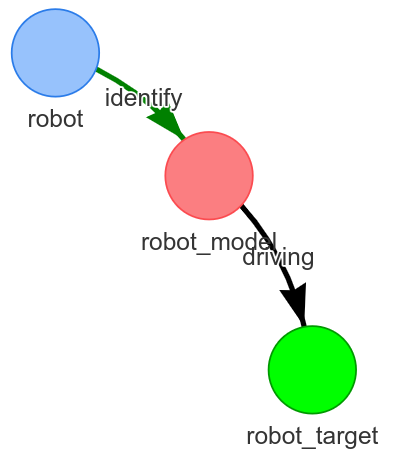
\includegraphics[width=0.35\textwidth]{figures/proposed_method/connecting_nodes/robot_to_target/execute_robot_to_target_2}}
\end{figure}
  \end{center}
\end{frame}


\begin{frame}[fragile]{Proposed Method: H-Algorithm}
    \vspace{-1cm}
  \begin{center}
\begin{figure}
  \subfloat{ 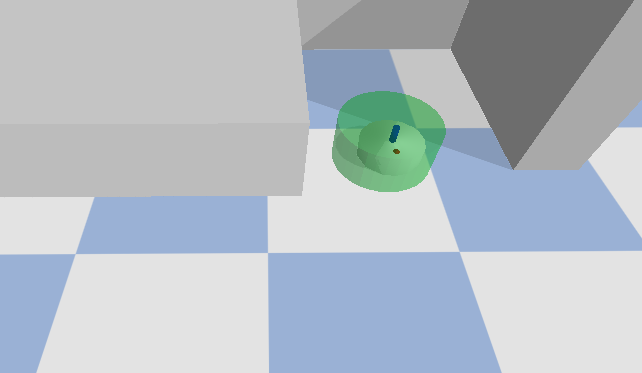
\includegraphics[width=0.45\textwidth]{figures/proposed_method/robot_to_target_ready}}\quad
  \subfloat{ 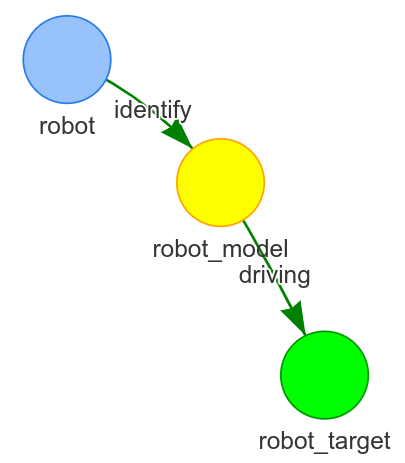
\includegraphics[width=0.35\textwidth]{figures/proposed_method/connecting_nodes/robot_to_target/execute_robot_to_target_3}}
\end{figure}
  \end{center}
\end{frame}

\begin{frame}[fragile]{Required Background} 
  \movie[width=\textwidth, height=0.4838\textwidth, autostart, poster]{}{figures/proposed_method/robot_to_target.mp4}
\end{frame}

\begin{frame}[fragile]{Proposed Method}
\vspace{-0.6cm}

\begin{center}
\begin{tikzpicture}[scale=0.75, every node/.style={scale=0.75}, node distance = 2cm, auto]

  \node [outer sep=0cm] (environment) at (0,0)  {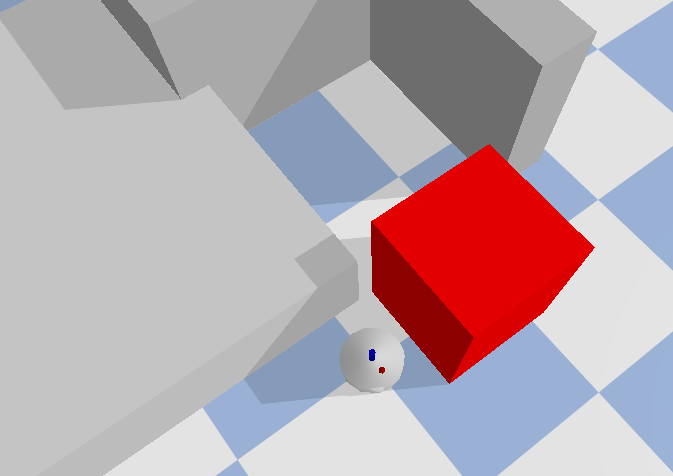
\includegraphics[width=4.6cm]{figures/introduction/robot_no_target}};

  \draw [myEvenLighterColor,
  rounded corners=0.3cm,
  line width=0.3cm]
  (environment.north west) --
  (environment.north east) --
  (environment.south east) --
  (environment.south west) -- cycle  ;

  \node [block,
  above of=environment,
  minimum height=2cm,
  minimum width=5cm,
  node distance=4.1cm,
  outer sep=0cm] (hgraph) {Hypothesis Algorithm};

  \node [block,
  above of=hgraph,
  node distance=3.3cm,
  minimum width=5cm,
  minimum height=2.0cm] (kgraph) {Knowledge Graph};

  % Draw edges
  \draw[-stealth] ([yshift=0.155cm, xshift=0.4 cm]environment.north) -- node [xshift=-.05cm, right] {\shortstack[]{sensor\\measurements}}([xshift=0.4 cm]hgraph.south) ;
  \draw[-stealth] ([xshift=-0.4 cm]hgraph.south) -- node [left] {robot input}([yshift=0.155cm, xshift=-0.4 cm]environment.north) ;
  \draw[stealth-] (hgraph.west) -- node [above] {task} ++(-1, 0);


  \draw[-stealth] ([xshift=-0.4cm]kgraph.south) -- node [left] {\shortstack[]{action\\suggestions}}([xshift= -0.4cm]hgraph.north) ;
  \draw[stealth-] ([xshift=0.4cm]kgraph.south) -- node [right] {\shortstack[]{action\\feedback}}([xshift= 0.4cm]hgraph.north) ;
\end{tikzpicture}
\end{center}

\end{frame}

\begin{frame}[fragile]{}
  % \vspace{-1.3cm}
  \begin{center}
    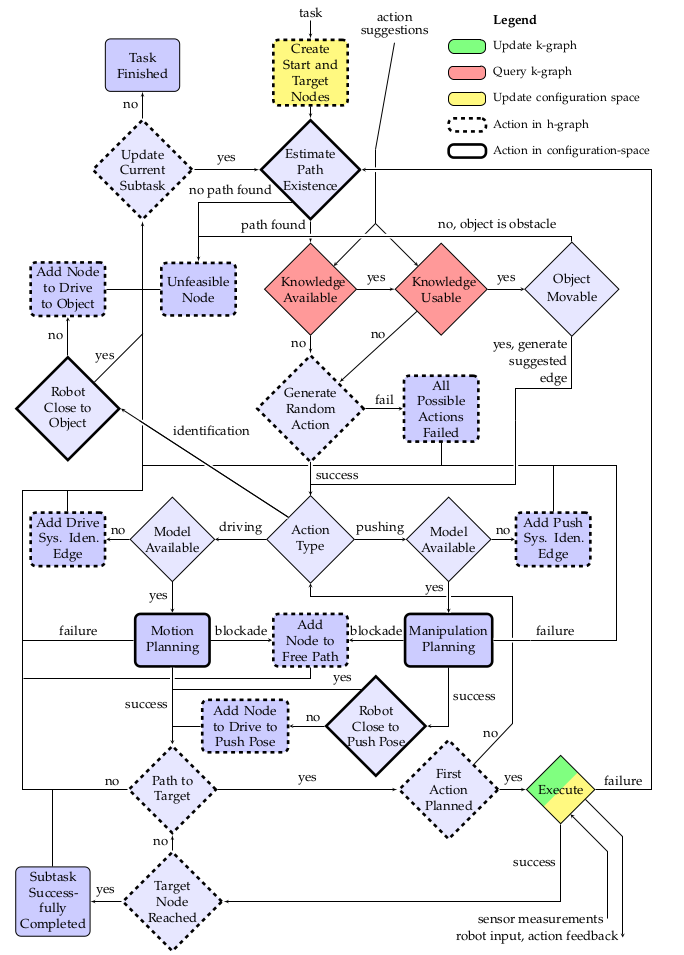
\includegraphics[height=0.95\textheight]{figures/proposed_method/tikz_flowchart_halgorithm}
  \end{center}
\end{frame}

\begin{frame}[fragile]{} 
  % \vspace{-1.3cm}
  \begin{center}
    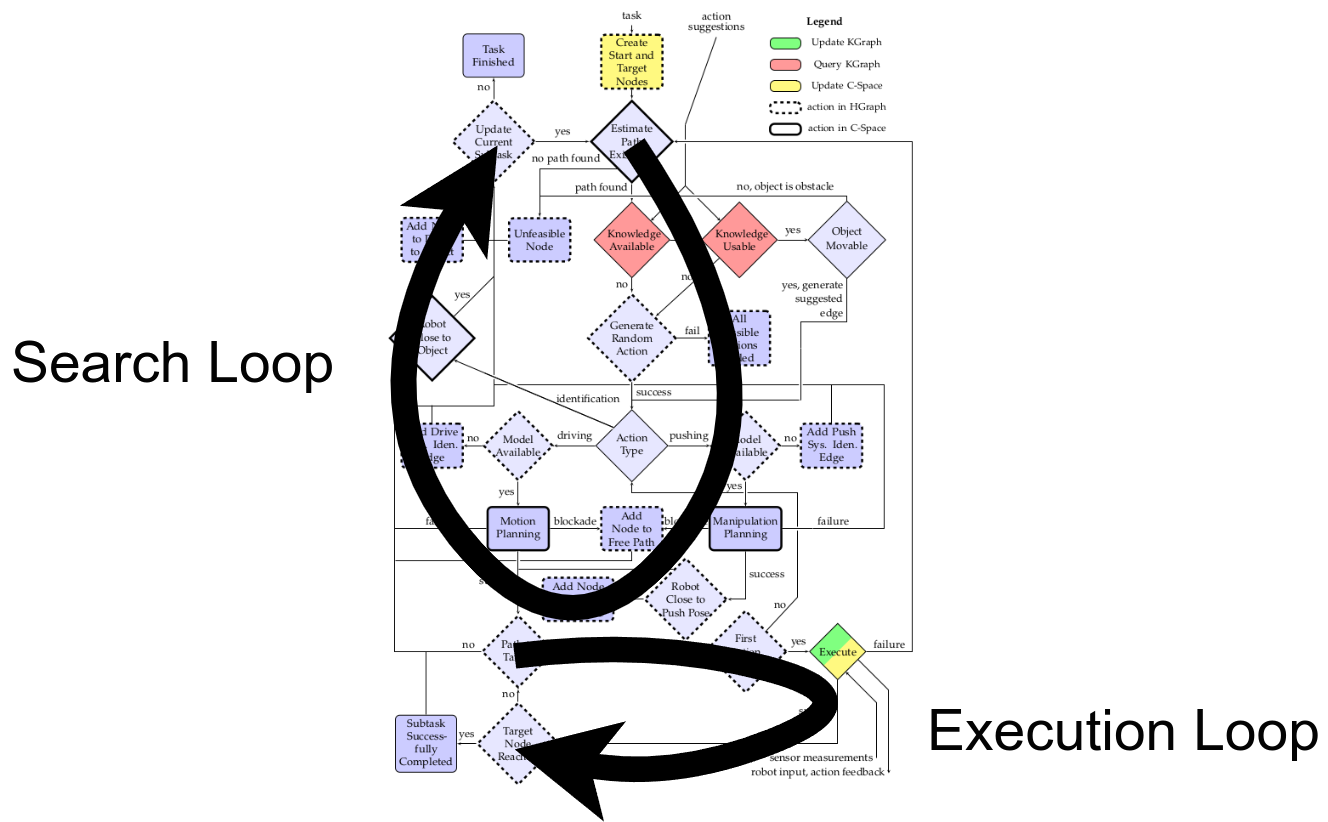
\includegraphics[height=0.98\textheight]{figures/proposed_method/two_loops_identified}
  \end{center}
\end{frame}


% \begin{frame}[fragile]{Proposed Method: H-Algorithm} 
%   \begin{center}
%     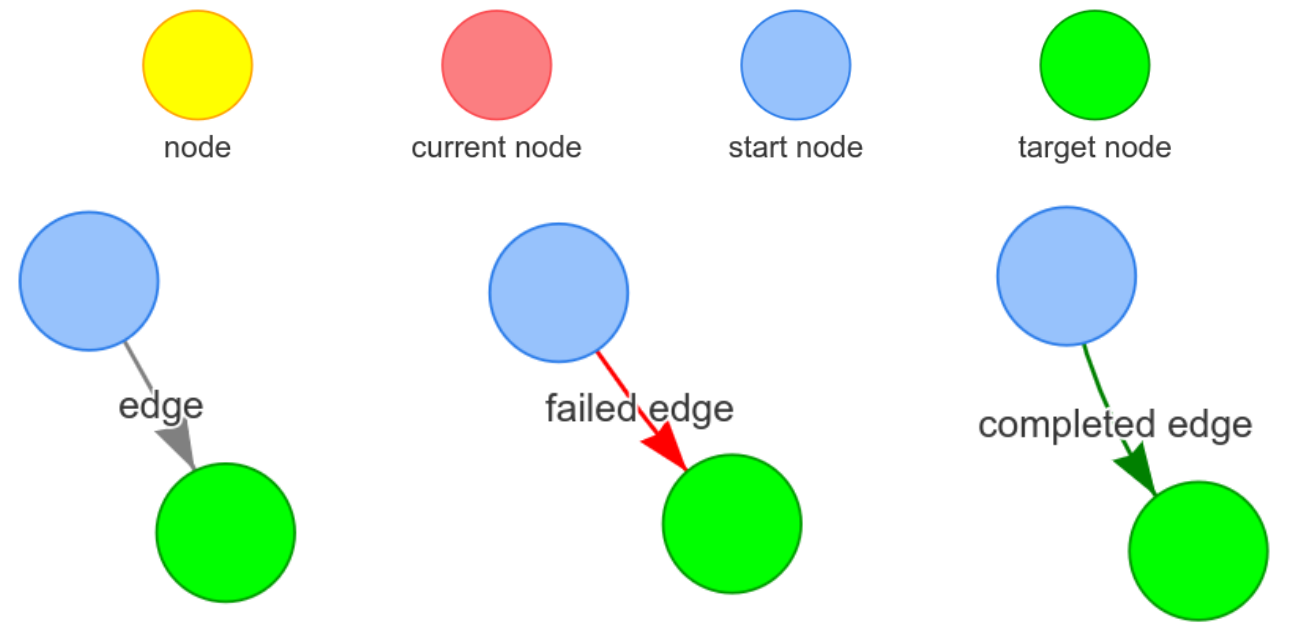
\includegraphics[width=1.0\textwidth]{figures/proposed_method/hgraph_legend}
%   \end{center}
% \end{frame}


% \begin{frame}[fragile]{Proposed Method: H-Algorithm} 
% \begin{center}
%   \todo{make a push a box image}
% \end{center}
% \end{frame}

% \begin{frame}[fragile]{Proposed Method: H-Algorithm} 
% \begin{center}
%   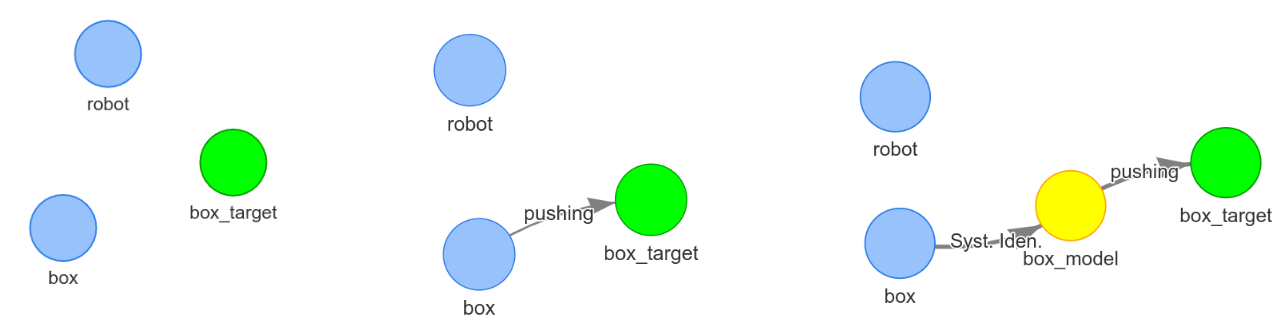
\includegraphics[width=1.0\textwidth]{figures/proposed_method/hgraph_example1}\pause

%   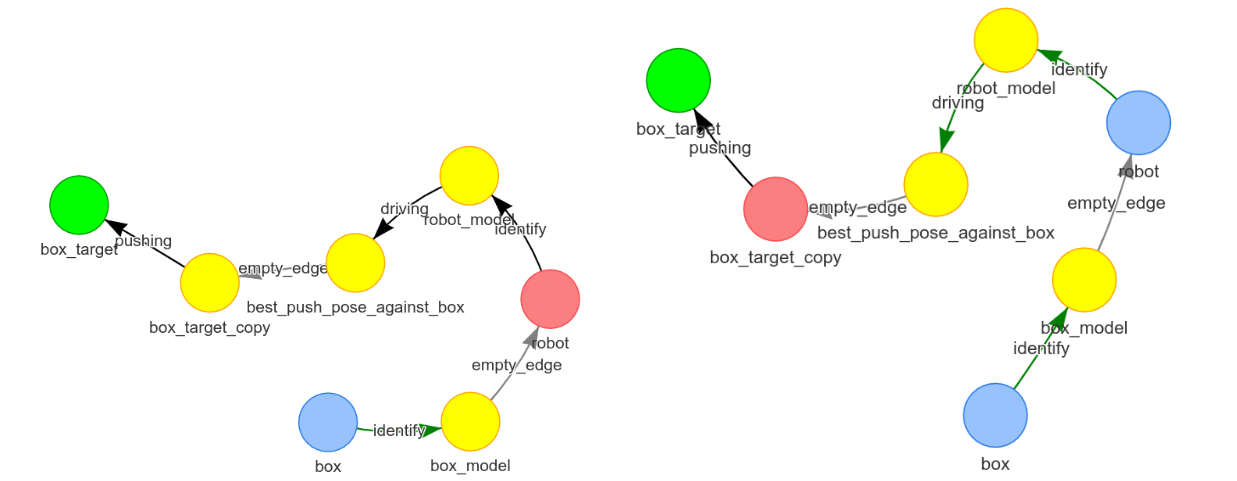
\includegraphics[width=1.0\textwidth]{figures/proposed_method/hgraph_example2}
% \end{center}
% \end{frame}

% \begin{frame}[fragile]{Proposed Method: H-Algorithm} 
%   \begin{center}
%     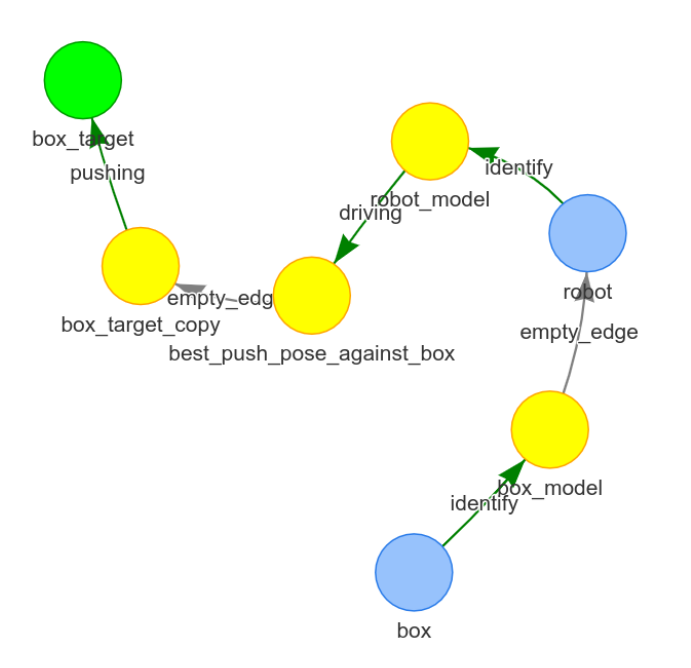
\includegraphics[width=0.5\textwidth]{figures/proposed_method/hgraph_example3}
%   \end{center}
% \end{frame}

\begin{frame}[fragile]{Proposed Method: H-Algorithm} 
\begin{block}{H-Algorithm behaviour}
    \begin{itemize}
      \item Fault detection $\rightarrow$ fail edge
      \item Blocking obstacle $\rightarrow$ free path 
      \item Stop regeneration of failed edges $\rightarrow$ blocklist
    \end{itemize}
  \end{block}
\end{frame}
